\section{Introduction}
\label{sec:introduction}

Software tool support is generally recognized as one of the main reasons
hindering the wider adoption of asynchronous design by the
industry~\cite{kondratyev2002design}\cite{nowick2015asynchronous}. Even~though
asynchronous design is based on rigorous theoretical foundations and has clear
advantages, its isolated ecosystem of flows, tools and formalisms presents a
formidable entry barrier to industrial users. It also introduces complexities
in designing modern multi-clock and Globally Asynchronous Locally Synchronous
Systems where pipelines, handshake circuits and other forms of asynchronous
``glue logic'' are used everywhere and expected to operate correctly with
their synchronous neighbors.

One of the challenges with integrating synchronous and asynchronous (further
referred to as ``sync'' and ``async'') components is performing system-level
verification. While the independent sync and async verification flows and
tools are mature and capable of verifying (sync or async) modules
independently, verifying a~mixed-timing sync-async system as a whole is
non-trivial. Due to the separation of the two flows, compatible behavioral
models of the sync/async parts of the system must be created and used to
verify each other (\Cref{fig_overview}a). For example, the sync part can be
coded as a~Signal Transition Graph (STG) to be made compatible with STG-based
asynchronous verification tools. This way, the sync/async implementations will
be verified against the environmental models of their counter-parts, but the
faithfulness of the models themselves will not be verified.

Based on the aforementioned, we argue that there is much value to be gained
from being able to verify asynchronous circuits using synchronous design
tools. First, this would enable designers to verify a mixed sync-async system
as a whole, overcoming the need for environmental models. Second, it will
simplify the verification process by unifying two independent flows. Third, it
will address the wider issue of EDA tool support for asynchronous circuit by
giving designers, particularly in industrial contexts, the option to use more
familiar or trusted tools. While we know there are no fundamental reasons
preventing the co-simulation (and consequently the verification) of mixed
sync-async systems~\cite{milner1980relating, milner1983calculi}, how and to
what degree does this work in practice remain open questions.

% fig_overview

\begin{figure}[!t]
\begin{center}

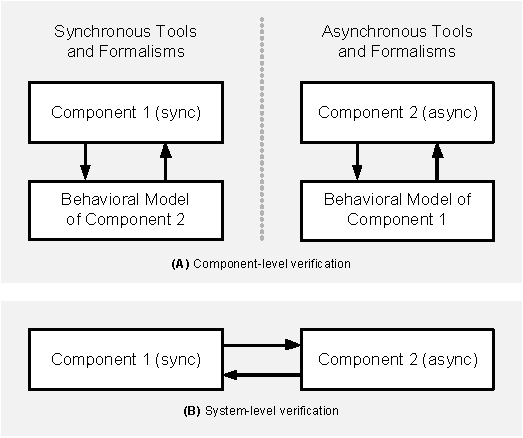
\includegraphics[width=8.8cm]{figures/fig_overview}

\caption{
Two approaches for verifying a mixed-timing system composed of a synchronous and asynchronous components. \textbf{(A)}~The sync/async components are verified independently using behavioral models of their counterparts. \textbf{(B)}~Both implementations are verified against each other directly.
}

\label{fig_overview}
\end{center}

\end{figure}


% fig_transformation

\begin{figure*}[!t]
\begin{center}

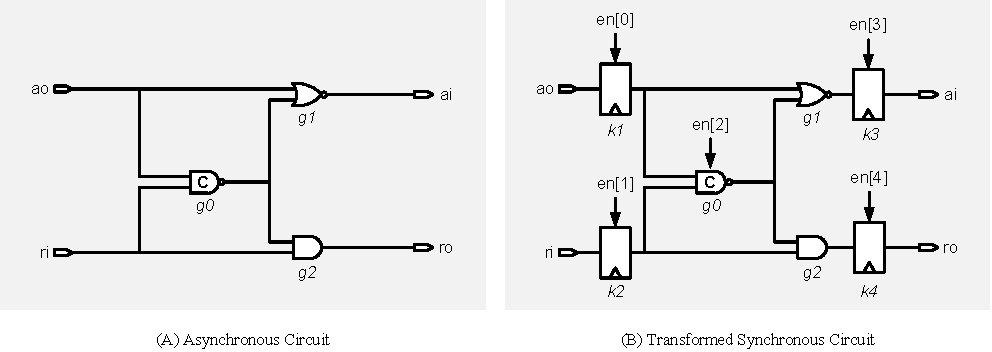
\includegraphics[width=17cm]{figures/fig_transformation}

\caption{
Proposed transformation to create a synchronous model of an asynchronous circuit. Flip-flops are inserted at inputs and gate outputs to capture net states, and corresponding signals~(\texttt{en}) simulate transitions by enabling (up to) one flip-flop at a time.
}

\label{fig_transformation}
\end{center}

\end{figure*}


\subsection{Main Idea}

We propose a simple transformation to convert gate-level asynchronous circuits
into clocked (synchronous) correspondents that can be verified using
synchronous design tools.\footnote{See \Cref{subsec:related} for related work
that exploits the same idea.} Briefly, we insert flip-flops at asynchronous
gate outputs and enable them one at a time to simulate transition firing. The
created synchronous model is then used by a formal tool to explore the
circuit's state space and verify its behavior.

\subsection{Contributions}

The contributions of this paper are as follows. (i) We propose a
transformation to convert asynchronous circuits into synchronous models, and
describe methods to encode and check correctness properties using these models
with synchronous verification tools. (ii) We report the results of using this
methodology with industrial and academic verification tools for synchronous
logic, cross-validating the results with \mpsat{} \cite{khomenko2006logic} and
a~custom tool (ESSET) which we developed for this purpose. (iii) We present
a~verification flow and use case example of mixed sync-async verification.
Finally, (iv)~we compare verification performance across three of the tools
using a~number of benchmark circuits.
